\documentclass[11pt,a4paper]{article}

\usepackage[margin=2.5cm]{geometry}
\usepackage{graphicx}
\usepackage{booktabs}
\usepackage{caption}
\usepackage{subcaption}
\usepackage{amsmath}
\usepackage{hyperref}
\usepackage{microtype}
\usepackage{parskip}
\usepackage[T1]{fontenc}
\usepackage[utf8]{inputenc}
\usepackage{lmodern}
\usepackage{xcolor}
\usepackage{enumitem}

\hypersetup{
    colorlinks=true,
    linkcolor=blue!60!black,
    citecolor=blue!60!black,
    urlcolor=blue!60!black,
}

% -------------------------------------------------------
\title{%
  \textbf{Stories We Tell (and the Machines Retell)}\\[0.4em]
  \large Cross-Cultural Narrative Structure in Llama~3.1~8B\\[0.6em]
  \normalsize NLP Final Project P12\\
  Università degli Studi di Milano\\
  Course: Natural Language Processing --- Prof.\ Alfio Ferrara
}
\author{Areg Karapetian}
\date{July 2026}
% -------------------------------------------------------

\begin{document}
\maketitle

% -------------------------------------------------------
\begin{abstract}
This project investigates whether a large language model preserves the
\emph{structure} of a folktale when asked to retell it ``in the style of'' a
different cultural tradition.  Starting from a corpus of 30 folktales drawn
equally from three traditions: European, Asian, and African~Diaspora. We
use Llama~3.1~8B (served locally via Ollama) to produce 60 cultural
retellings.  Each story version is converted into a \emph{narrative graph}
in which characters and objects are nodes and plot events are directed, labelled
edges.  We compare originals against retellings along four complementary
dimensions: graph edit distance, relational motif overlap, character-role
alignment, and sentence-embedding cosine similarity.  Results show that (i)~the
original stories do not cluster cleanly by culture, suggesting shared structural
archetypes; (ii)~European-style retellings diverge most from the originals
structurally; and (iii)~African~Diaspora-style retellings are closest to the
originals on every metric, suggesting the model imposes weaker stylistic
changes when targeting that tradition.
\end{abstract}

% -------------------------------------------------------
\section{Introduction}

Folktales are one of the most studied objects in computational narratology
\cite{propp1928,bremond1966}: they are short, self-contained, and exhibit
recurring structural patterns that cross cultural boundaries.  At the same time,
each cultural tradition inflects those patterns in characteristic ways through
the choice of characters, the type of conflict, and the nature of the resolution.

Large language models such as Llama~3.1~8B have absorbed vast multilingual text,
including folktale collections, mythologies, and literary adaptations.  When
such a model is instructed to retell a story ``in the style of'' a particular
cultural tradition, two outcomes are possible.  Either the model reproduces the
deep narrative structure faithfully while only adjusting surface elements (names,
settings, vocabulary), or it restructures the plot itself in culturally typical
ways.  Distinguishing between these two outcomes requires a structural, not merely
lexical, comparison.

This project operationalises that comparison through narrative graphs and four
structural metrics, applied uniformly across 90 story versions (30 originals and
60 retellings).  The pipeline combines prompt engineering with structured JSON
output, local LLM inference via Ollama, and transformer-based sentence
embeddings for semantic similarity.

% -------------------------------------------------------
\section{Dataset}

The corpus consists of 30 English-language folktales, 10 per cultural tradition:
\textbf{European}, \textbf{Asian}, and \textbf{African~Diaspora}.  All texts are
drawn from public-domain collections published before~1930 (e.g.\ Fansler's
\textit{Filipino Popular Tales}, Bompas's \textit{Folklore of the Santal
Parganas}, and Carey's \textit{Fairy Legends of the French Provinces}).
Story lengths range from roughly 320 to 900 words; the median is approximately
560 words.

Each of the 30 originals is retold into the two \emph{other} cultural styles,
yielding 60 retellings and a total of 90 story versions.  Because the entire
pipeline runs in English on a single local model, cross-lingual effects are
deliberately excluded.

% -------------------------------------------------------
\section{Methodology}

\subsection{Retelling with Llama~3.1~8B}

Retellings are generated by \texttt{src/retell\_all.py} using zero-shot prompting:
\begin{quote}
\textit{Retell the following folktale in the style of \{target\} folktales.\\
Keep the SAME main events and the SAME ending.\\
Do NOT add new major plot points.\\
Output ONLY the retold story text.  No title.  No explanations.}
\end{quote}
Temperature is set to~0.35 to allow stylistic variation while limiting
hallucination; if the output is shorter than 200 words, up to two retries are
made at higher temperatures (0.55, then 0.6).  Each retelling targets a word
count within~$\pm15\%$ of the original.  For the African~Diaspora target, the
prompt additionally requires Standard English and forbids dialect or
phonetic-spelling imitation, so that cultural style is expressed through themes,
imagery, and oral-storytelling cadence rather than caricature.  Ollama is used
as the inference backend, communicating with the model via its local REST API.

\subsection{Event Extraction}

\texttt{src/extract\_events\_all.py} prompts the same model (temperature~0.2) to
produce a JSON list of 10--14 chronological plot events per story version.  The
prompt enforces a strict schema:

\begin{verbatim}
{ "events": [ {"i": 1, "event": "..."}, ... ] }
\end{verbatim}

A two-stage fallback handles malformed outputs: a retry with a stricter reminder
prompt, followed by a regex parser that recovers event strings directly from
partially-formed JSON.  The output file \texttt{events\_final.jsonl} contains 90
records covering all story versions.

\subsection{Narrative Graph Construction}

\texttt{src/extract\_triples.py} converts each event list into (subject,
relation, object) triples, again via structured LLM prompting.  The relation
phrase is constrained to 2--4 lowercase words, entity labels are normalised
(articles stripped, lowercased), and the same character must receive the same
label throughout a story.

\texttt{src/build\_graphs.py} assembles these triples into directed multigraphs
(NetworkX \texttt{MultiDiGraph}).  Events with no clear object become self-loops.
Within each story version, the entity appearing as subject most frequently is
labelled \textsc{Protagonist}; the runner-up is \textsc{Deuteragonist};
everything else is \textsc{Other}.

From each graph we extract eight structural features: node count, edge count,
self-loop count, distinct relation count, average out-degree, maximum out-degree,
graph density, and number of weakly connected components.

\subsection{Metrics}

Four metrics compare an original story to each of its retellings:

\paragraph{Normalised graph edit distance (GED).}
We compute \texttt{networkx.graph\_edit\_distance} on the unlabelled digraphs
(collapsing parallel edges) and normalise by
$\max(|V|+|E|)$ so scores are comparable across stories of different lengths.
A timeout of 10~seconds is imposed; unresolved pairs are excluded.

\paragraph{Relation/motif overlap.}
Jaccard similarity between the sets of action words in the original's and
retelling's relation phrases (stop-words removed).

\paragraph{Role alignment.}
For each event position up to $\min(|S_1|,|S_2|)$, we compare whether
the subject (and separately, the object) carries the same role label
(\textsc{Protagonist}, \textsc{Deuteragonist}, or \textsc{Other}) in both
versions.  The score is the fraction of matching positions.

\paragraph{Semantic similarity.}
We encode each full story text with
\texttt{all-MiniLM-L6-v2}~\cite{reimers2019sentence}, a BERT-based sentence
encoder, and report the cosine similarity between the
original and the retelling embeddings.  This metric captures meaning-level
preservation independently of graph structure.

% -------------------------------------------------------
\section{Results}

\subsection{Clustering of Original Stories}

\begin{figure}[h]
  \centering
  \begin{subfigure}[b]{0.48\textwidth}
    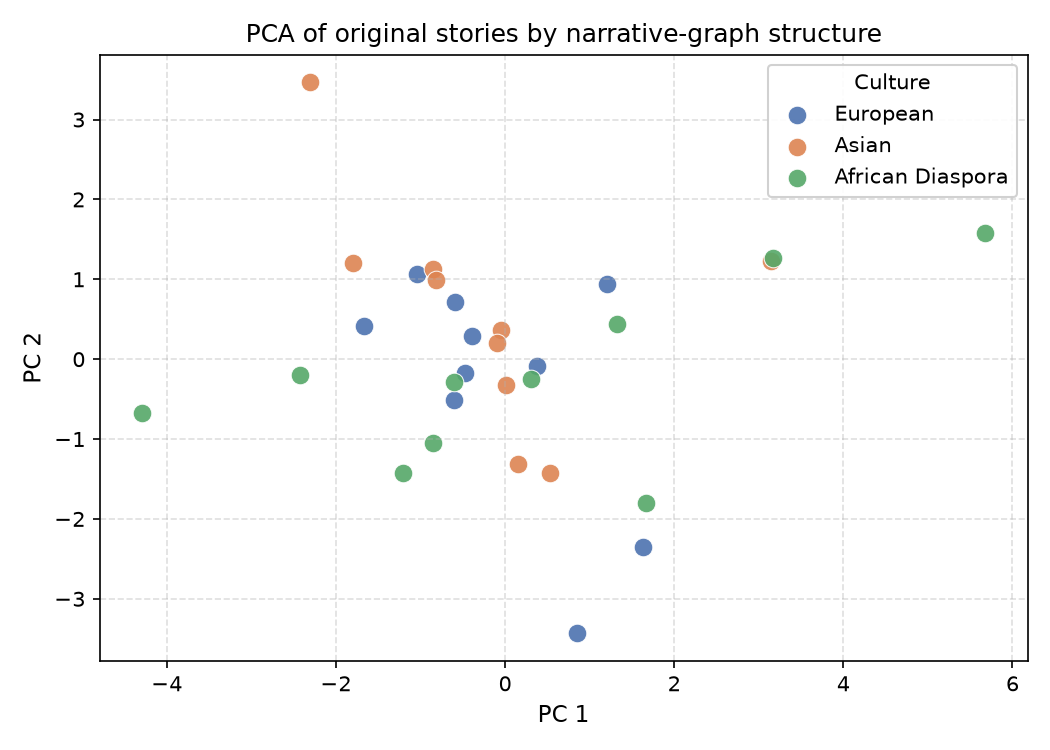
\includegraphics[width=\textwidth]{results/analysis/pca_stories.png}
    \caption{PCA of the 8 structural graph features (originals only).}
    \label{fig:pca}
  \end{subfigure}
  \hfill
  \begin{subfigure}[b]{0.48\textwidth}
    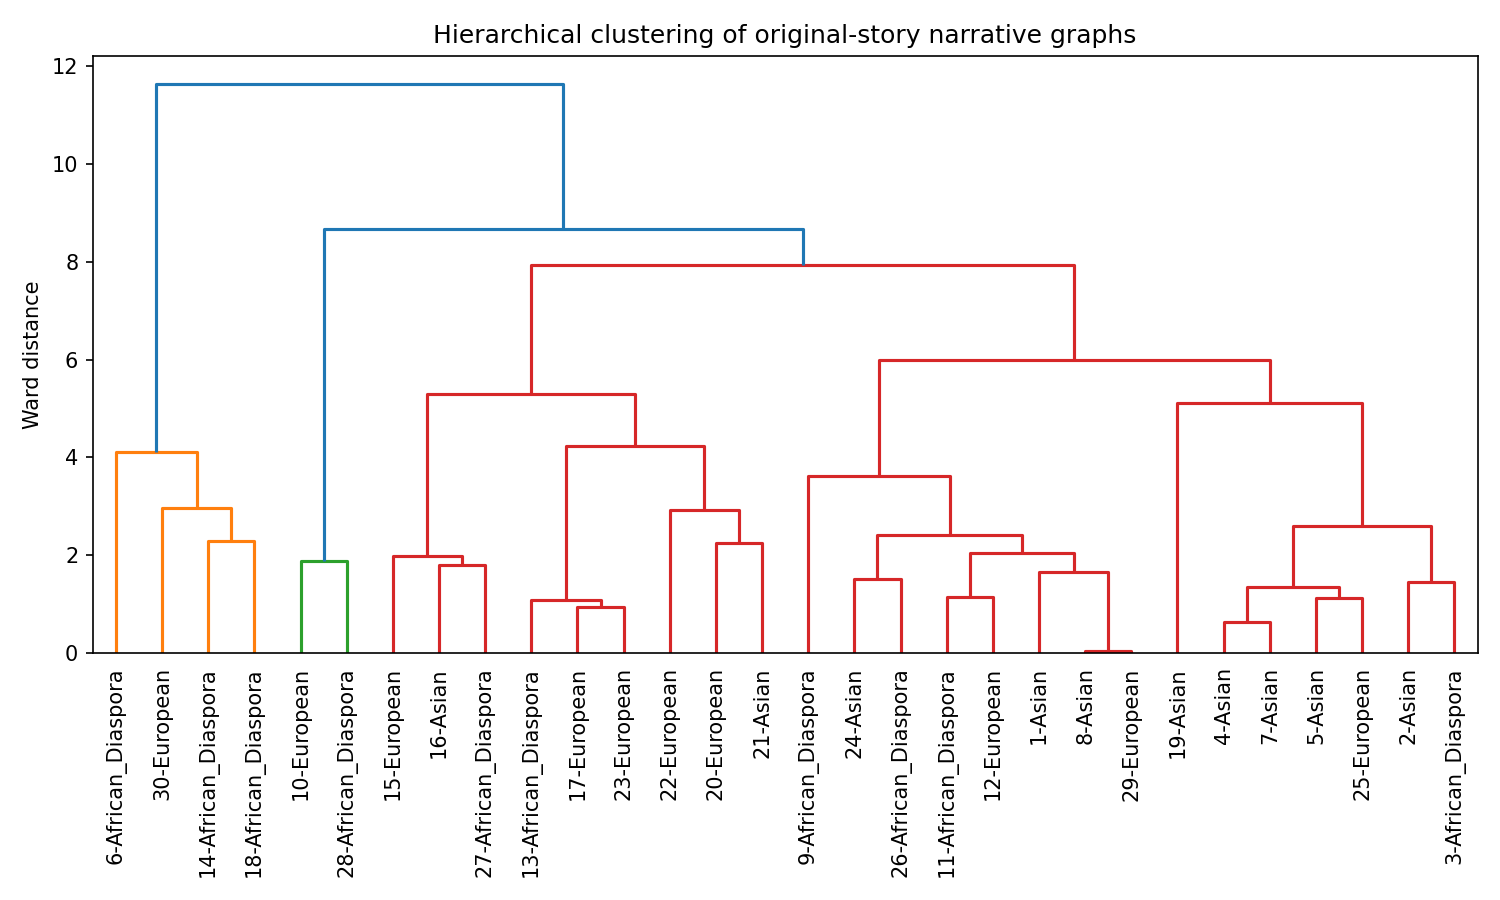
\includegraphics[width=\textwidth]{results/analysis/dendrogram.png}
    \caption{Hierarchical clustering dendrogram (Ward linkage).}
    \label{fig:dendro}
  \end{subfigure}
  \caption{Structure of the original-story space.  In~(a) colours indicate
           cultural tradition; in~(b) leaf labels give story id and culture.
           Neither K-Means ($k{=}3$) nor hierarchical clustering recovers
           clean culture-level groups.}
  \label{fig:clustering}
\end{figure}

\autoref{fig:clustering} shows the structural feature space of the 30 original
stories.  K-Means ($k{=}3$) assigns 14, 13, and 3 stories to the three
clusters, none of which aligns with a single culture
(\autoref{tab:kmeans}).  The dominant cluster (14 stories) contains 6 Asian,
6 European, and 2 African~Diaspora texts.  Hierarchical clustering (Ward linkage)
produces a similarly mixed dominant group of 21 stories
(\autoref{tab:hier}).  These results provide mild evidence for universal
narrative archetypes: at the level of simple graph statistics, folktales from
different traditions occupy the same structural space.

\begin{table}[h]
  \centering
  \begin{subtable}[t]{0.45\textwidth}
    \centering
    \begin{tabular}{lccc}
      \toprule
      Cluster & Eur. & Asian & A.D. \\
      \midrule
      0 & 6 & 6 & 2 \\
      1 & 4 & 3 & 6 \\
      2 & 0 & 1 & 2 \\
      \bottomrule
    \end{tabular}
    \caption{K-Means ($k{=}3$).}
    \label{tab:kmeans}
  \end{subtable}
  \hfill
  \begin{subtable}[t]{0.45\textwidth}
    \centering
    \begin{tabular}{lccc}
      \toprule
      Cluster & Eur. & Asian & A.D. \\
      \midrule
      1 & 7 & 8 & 6 \\
      2 & 2 & 1 & 1 \\
      3 & 1 & 1 & 3 \\
      \bottomrule
    \end{tabular}
    \caption{Hierarchical / Ward ($k{=}3$).}
    \label{tab:hier}
  \end{subtable}
  \caption{Culture breakdown per cluster for the 30 original stories.
           A.D.\ = African~Diaspora.}
\end{table}

\subsection{Cross-Cultural Structural Comparison}

\begin{figure}[h]
  \centering
  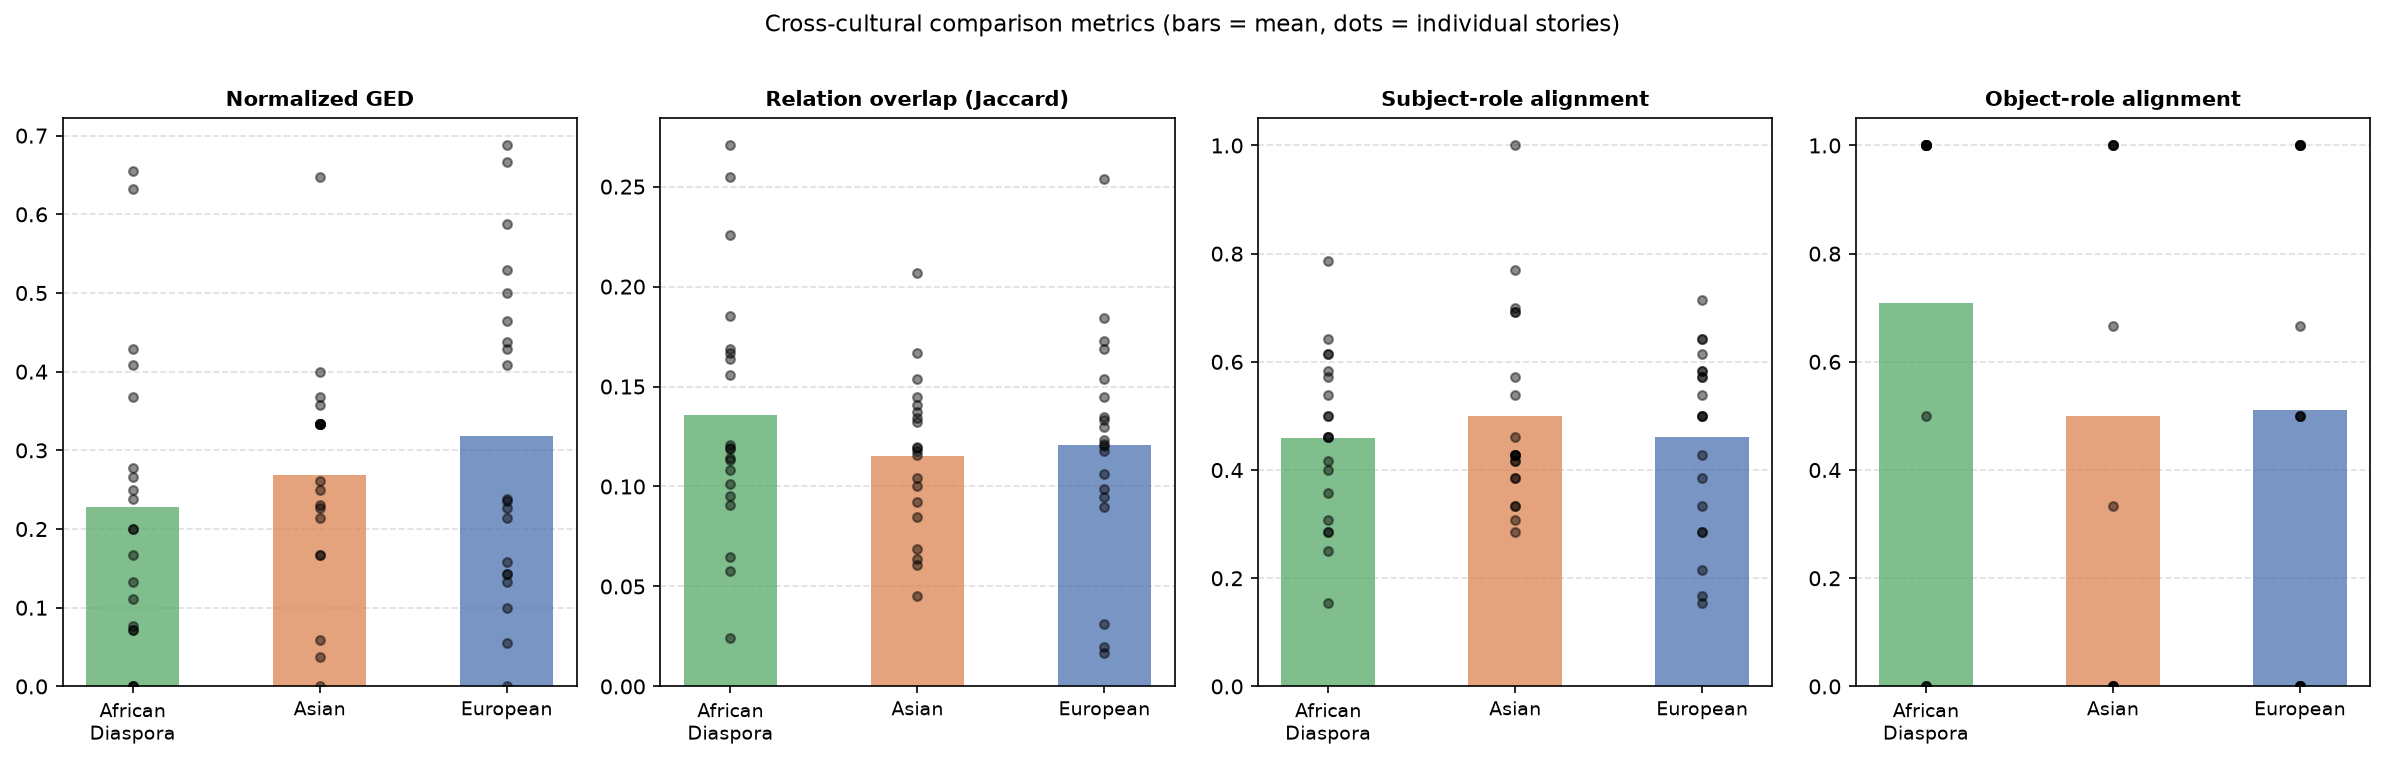
\includegraphics[width=\textwidth]{results/analysis/comparison_by_culture.png}
  \caption{Four structural metrics by target culture.  Bars show the mean;
           dots show individual story pairs.}
  \label{fig:comparison}
\end{figure}

\autoref{tab:metrics} summarises the four metrics averaged over all story pairs
for each target culture; \autoref{fig:comparison} shows the distributions.

\begin{table}[h]
  \centering
  \begin{tabular}{lcccc}
    \toprule
    Target culture & Norm.\ GED & Rel.\ overlap & Subj.\ align. & Obj.\ align. \\
    \midrule
    African~Diaspora & \textbf{0.228} & \textbf{0.136} & 0.460 & \textbf{0.708} \\
    Asian            & 0.269          & 0.115          & \textbf{0.500} & 0.500 \\
    European         & 0.318          & 0.121          & 0.461 & 0.512 \\
    \bottomrule
  \end{tabular}
  \caption{Cross-cultural comparison metrics (means across 20 story pairs per
           target culture).  Bold marks the best value per column.
           Lower GED = closer to original; higher overlap/alignment = closer.}
  \label{tab:metrics}
\end{table}

Three findings stand out.

\textbf{European retellings diverge most.}  The normalised GED for European
retellings (0.318) is substantially higher than for African~Diaspora (0.228)
and Asian (0.269) retellings, indicating that the model restructures the
narrative graph most aggressively when targeting a European style.

\textbf{African~Diaspora retellings stay closest.}  This culture has the
lowest GED, the highest relation overlap, and the highest object-role alignment
(0.708).  The model appears to make smaller structural changes when retelling in
an African~Diaspora style, possibly because the training distribution for that
style is closer to the source stories.

\textbf{Subject-role alignment is culture-invariant.}  Across all three target
cultures, the fraction of event positions where the protagonist role is preserved
hovers between 0.46 and 0.50.  The model consistently identifies \emph{who} the
story is about, regardless of the target style.  Cultural differences surface
mainly in secondary relationships (object-role alignment).

\autoref{fig:graphs} shows example narrative graphs for two original stories,
illustrating the range of extracted structures: story~9 yields a rich
multi-entity graph with many cross-entity edges, while story~1 is dominated by
self-loops (events with no clear object entity) and disconnected nodes a
known source of noise in LLM-extracted graphs.

\begin{figure}[h]
  \centering
  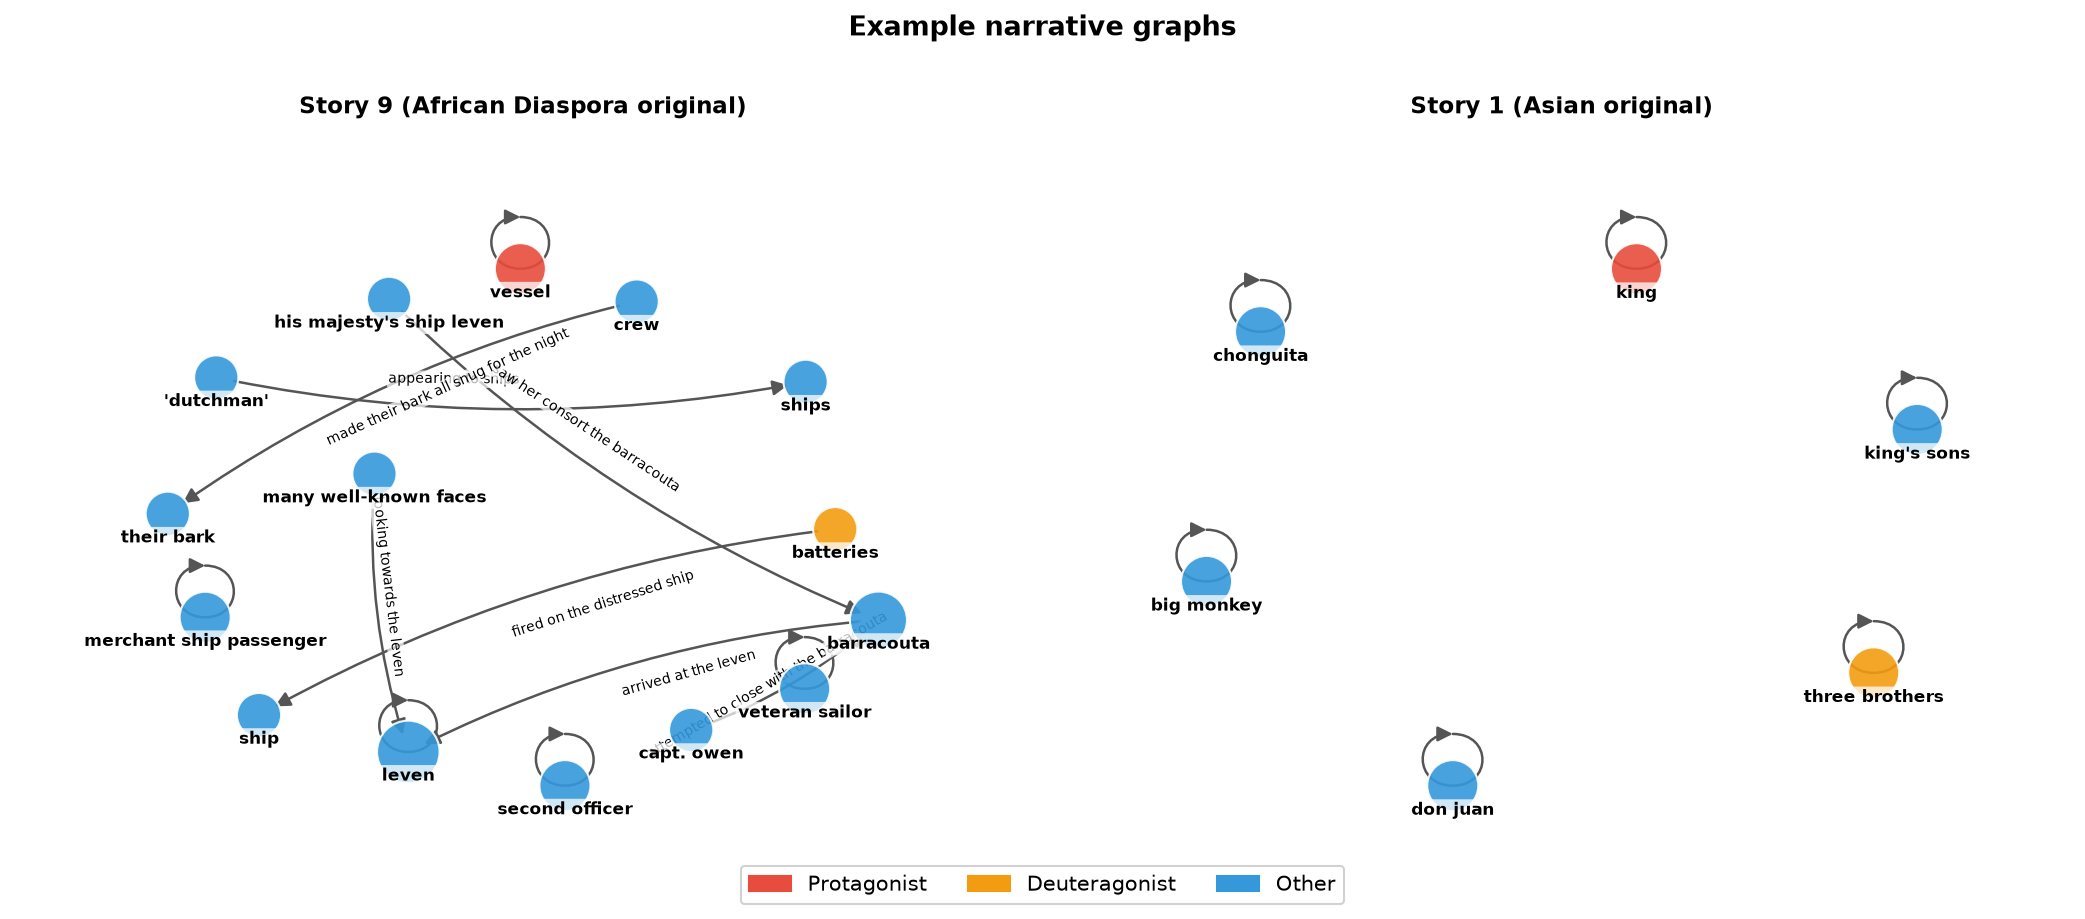
\includegraphics[width=0.82\textwidth]{results/analysis/example_graphs.png}
  \caption{Narrative graphs for two original stories.  Node colour indicates
           role: red = Protagonist, orange = Deuteragonist, blue = Other.
           Curved loop arcs are self-loops, i.e.\ events with no clear object
           entity.}
  \label{fig:graphs}
\end{figure}

\subsection{Semantic Similarity}

\begin{figure}[h]
  \centering
  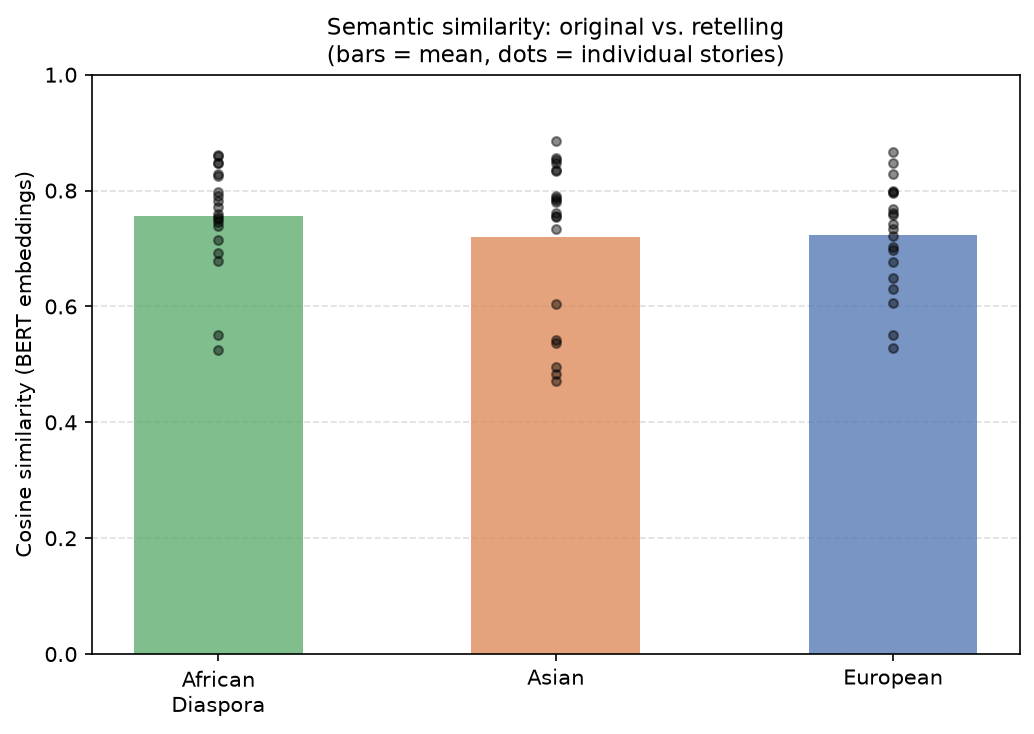
\includegraphics[width=0.55\textwidth]{results/analysis/semantic_similarity.png}
  \caption{BERT cosine similarity (all-MiniLM-L6-v2) between original and
           retelling texts.  Bars show the mean; dots show individual pairs.}
  \label{fig:semantic}
\end{figure}

\autoref{tab:semantic} and \autoref{fig:semantic} show semantic similarity
computed from sentence embeddings.

\begin{table}[h]
  \centering
  \begin{tabular}{lc}
    \toprule
    Target culture & Mean cosine similarity \\
    \midrule
    African~Diaspora & \textbf{0.756} \\
    European         & 0.723 \\
    Asian            & 0.720 \\
    \bottomrule
  \end{tabular}
  \caption{Mean BERT cosine similarity between original and retelling.}
  \label{tab:semantic}
\end{table}

The BERT results corroborate the graph-structural findings: African~Diaspora
retellings are the most semantically similar to their originals (0.756), while
European and Asian retellings are nearly indistinguishable from each other
(${\approx}0.72$).

A notable observation is the small \emph{spread} of the difference: 0.72 vs.\
0.76 is a modest gap, suggesting that on average the model does not drastically
alter the meaning of a story regardless of the target culture.  Individual
variation is substantial, however story~25 scores 0.47 to Asian but 0.79 to
African~Diaspora, while story~17 achieves 0.89 to Asian.  This variance
indicates that the model's cultural adaptation is story-dependent, not uniform.

% -------------------------------------------------------
\section{Discussion}

The clearest result is the asymmetry between target cultures in structural
divergence.  European-style retellings change narrative graphs most, while
African~Diaspora-style retellings change them least.  One interpretation is that
the model has less distinctive ``European folktale'' prior to draw on and
compensates by restructuring the plot; alternatively, the European style may
require more assertive changes to vocabulary and setting that indirectly
affect the graph.  Resolving this would require ablating the prompt or inspecting
the model's attention patterns with explainability techniques.

The clustering finding that original stories do not separate by culture is
itself informative.  Eight simple graph statistics are insufficient to distinguish
European from Asian from African~Diaspora folktales.  Either the cultural signal
lies in subtler structural features (motif sequences, character type distributions)
or the structural universality hypothesis has some empirical grounding even in
this small corpus.

The stability of subject-role alignment (protagonist identification) across
target cultures is reassuring: the model does not confuse \emph{who} the story
is about, even when it changes \emph{what} happens.  This is consistent with
findings in the LLM narrative generation literature that models reliably track
primary agents.

\subsection*{Limitations}

\begin{itemize}[noitemsep]
  \item \textbf{Small corpus.} 30 stories / 60 pairs is too few for statistical
    testing; reported values are descriptive trends.
  \item \textbf{English only.} All texts are in English, which may bias the
    model's cultural adaptations toward the most common English-language folktale
    conventions.
  \item \textbf{Single model.} Results apply specifically to Llama~3.1~8B and
    may not generalise to larger or differently-trained models.
  \item \textbf{LLM-extracted graphs.} Events, triples, and entity labels all
    come from single-pass Llama outputs with no human verification; some noise
    is expected.
  \item \textbf{GED approximation.} The 10-second timeout means that very large
    graph pairs may return an approximate rather than exact distance.
\end{itemize}

% -------------------------------------------------------
\section{Conclusions}

We presented a pipeline for comparing the narrative structure of folktale
originals and LLM retellings across three cultural traditions.  Using a
combination of narrative graphs and BERT sentence embeddings, we found that
Llama~3.1~8B preserves protagonist identity robustly across all target styles,
but diverges most in graph structure when targeting European styles and least
when targeting African~Diaspora styles.  Original stories, clustered by
graph-level features alone, do not separate by culture, hinting at shared
narrative archetypes.


% -------------------------------------------------------
\section*{AI Usage Disclaimer}

Parts of this project have been developed with the assistance of Antropic's Claude(Opus 4.8). The AI was used to support
the development of project ideas, the structuring of methodological workflows, the drafting of descriptive texts,
and the identification of relevant datasets and references. All content produced with AI assistance has been carefully
reviewed, edited, and validated by me. I take full responsibility for the final content and its accuracy, relevance, and
academic integrity.

% -------------------------------------------------------
\begin{thebibliography}{9}

\bibitem{propp1928}
V.~Propp (1928).
\textit{Morphology of the Folktale}.
Leningrad: Academia.

\bibitem{bremond1966}
C.~Br\'{e}mond (1966).
``La logique des possibles narratifs.''
\textit{Communications}, 8, 60--76.

\bibitem{reimers2019sentence}
N.~Reimers and I.~Gurevych (2019).
``Sentence-BERT: Sentence Embeddings using Siamese BERT-Networks.''
\textit{Proceedings of EMNLP 2019}.

\bibitem{ollama}
Ollama (2024).
\textit{Ollama: Run Large Language Models Locally}.
\url{https://ollama.com/}

\bibitem{llama3}
Meta AI (2024).
\textit{Llama~3.1 Model Card}.
\url{https://ai.meta.com/blog/meta-llama-3/}

\bibitem{networkx}
A.~Hagberg, P.~Swart, and D.~Schult (2008).
``Exploring Network Structure, Dynamics, and Function using NetworkX.''
\textit{Proceedings of the 7th Python in Science Conference}.

\end{thebibliography}

\end{document}
